\documentclass[tikz,border=10pt]{standalone}
\begin{document}
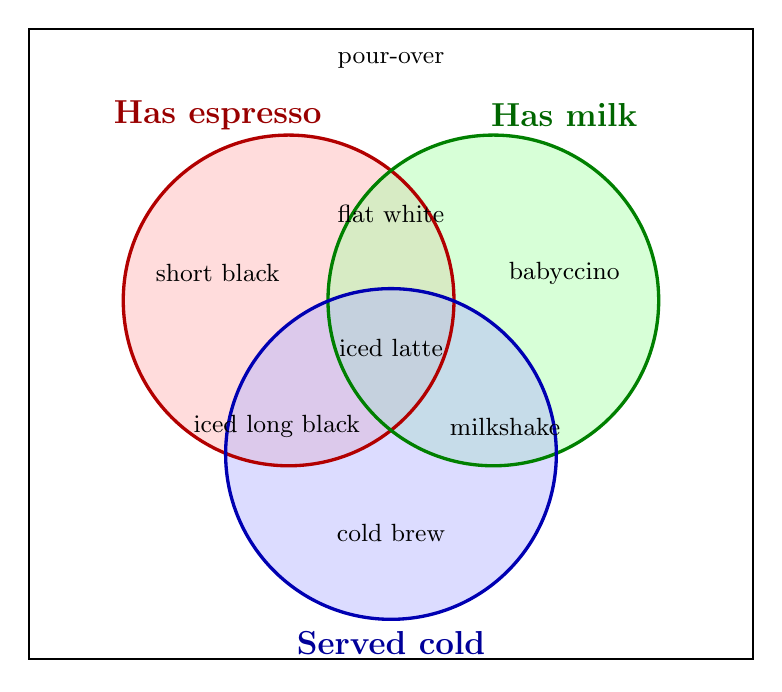
\begin{tikzpicture}[thick]
  % Bounding box
  \draw (-4.6,-3.8) rectangle (4.6,4.2);

  % Circles
  \begin{scope}
    \fill[red!30,   fill opacity=0.45] (-1.3, 0.75) circle (2.1);
    \fill[green!35, fill opacity=0.45] ( 1.3, 0.75) circle (2.1);
    \fill[blue!30,  fill opacity=0.45] ( 0.0,-1.20) circle (2.1);
  \end{scope}
  \draw[red!70!black,   very thick] (-1.3, 0.75) circle (2.1);
  \draw[green!50!black, very thick] ( 1.3, 0.75) circle (2.1);
  \draw[blue!70!black,  very thick] ( 0.0,-1.20) circle (2.1);

  % Circle labels
  \node[red!60!black,   font=\bfseries\large] at (-2.2, 3.1) {Has espresso};
  \node[green!40!black, font=\bfseries\large] at ( 2.2, 3.1) {Has milk};
  \node[blue!60!black,  font=\bfseries\large] at ( 0.0,-3.6) {Served cold};

  % Drinks
  \node[font=\small] at (-2.2, 1.1)  {short black};      % espresso only
  \node[font=\small] at ( 2.2, 1.1)  {babyccino};        % milk only
  \node[font=\small] at ( 0.0,-2.2)  {cold brew};        % cold only
  \node[font=\small] at ( 0.0, 1.85) {flat white};       % espresso + milk
  \node[font=\small] at (-1.45,-0.85){iced long black};  % espresso + cold
  \node[font=\small] at ( 1.45,-0.85){milkshake};        % milk + cold
  \node[font=\small] at ( 0.0, 0.15) {iced latte};       % all three
  \node[font=\small] at ( 0.0, 3.8)  {pour-over};        % outside all
\end{tikzpicture}
\end{document}
